\documentclass[11pt, a4paper]{article}
\usepackage{amsmath, amsthm, amssymb, calrsfs, wasysym, verbatim, bbm, color, graphics, geometry}
\usepackage[utf8]{inputenc} % comment when using lualatex
\usepackage[italian]{babel} % lingua e a-capo-sillabato
\usepackage{fullpage}
\usepackage{graphicx}
%\usepackage[hidelinks]{hyperref,xcolor} % link di pagina
\usepackage[bottom]{footmisc} % note appiccicate al fondo della pagina
\usepackage{float} % per posizionamento immagini
\usepackage{cancel}

\geometry{tmargin=.75in, bmargin=.75in, lmargin=.75in, rmargin = .75in}  

\newcommand{\R}{\mathbb{R}}
\newcommand{\C}{\mathbb{C}}
\newcommand{\Z}{\mathbb{Z}}
\newcommand{\N}{\mathbb{N}}
\newcommand{\Q}{\mathbb{Q}}
\newcommand{\Cdot}{\boldsymbol{\cdot}}

\newtheorem{thm}{Theorem}
\newtheorem{defn}{Definition}
\newtheorem{conv}{Convention}
\newtheorem{rem}{Remark}
\newtheorem{lem}{Lemma}
\newtheorem{cor}{Corollary}



\definecolor{dkgreen}{rgb}{0,0.6,0}
\definecolor{gray}{rgb}{0.5,0.5,0.5}
\definecolor{mauve}{rgb}{0.58,0,0.82}


\title{Distributed Systems}
\author{Raffaele Castagna}

\date{Academic Year 2025-2026}

\begin{document}

\maketitle

\tableofcontents
\newpage

\section{Introduction}
\begin{defn}
    In a system we have \textit{n} processes in $\prod:{p_{0}\dots,p_{n-1}}$ each with a distinct identity
    they communicate by utilizing a communication graph \textbf{G : ($\prod,E$)}, the communication is done by exchanging messages.

\end{defn}
\begin{center}
    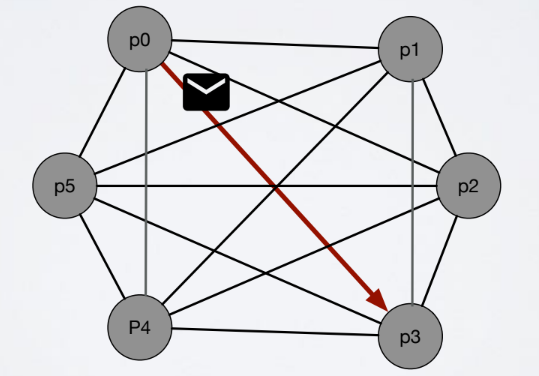
\includegraphics[scale=0.6]{img/comm graph}
\end{center}
\begin{defn}
A process is a (possibily infinite) State Machine (I/O Automaton).
\end{defn}
\begin{center}
    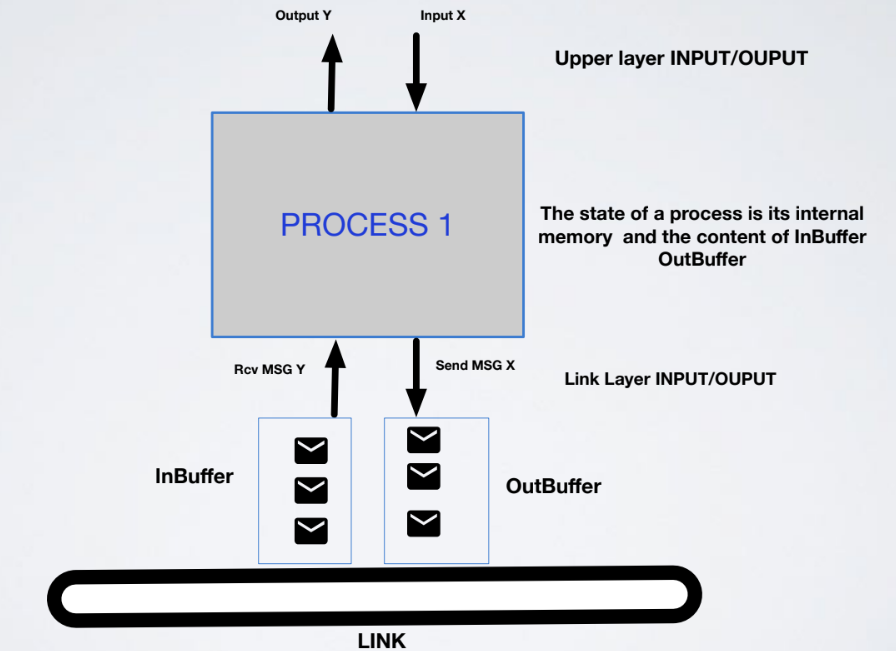
\includegraphics[scale=0.55]{img/process.png}
\end{center}
Each process has multiple qualities:
\begin{itemize}
    \item A set of internal states \textit{Q}
    \item A set of initial states $Q_i \subset Q$
    \item A set of all possible messages M in the form <sender,receiver,payload>
    \item Multiset of delivered messages $InBuf_j$
    \item Multiset of inflight messages $OutBuf_j$
\end{itemize}
\newpage
We can formally describe this as follows: (this isnt part of the exam btw) 
$$P_j (q \in Q \cup Q_{in},InBuf_j) = (q' \in Q, SendMsg \subset M \newline)$$  $$ OutBuf_j = OutBuf_j \cup SendMsg$$ $$\newline InBuf_j = \cancel{0}$$
To execute a process we have an adversary that schedules a set of events (scheduler), these events may be for example a delivery (e.g. Del(m,i,j)) or it can be one step of the step machine of process i (Exec(i))
\begin{defn}
    A configuration $C_t$ is a vector of n components, component j indicates the state of process j.
\end{defn}
\begin{center}
    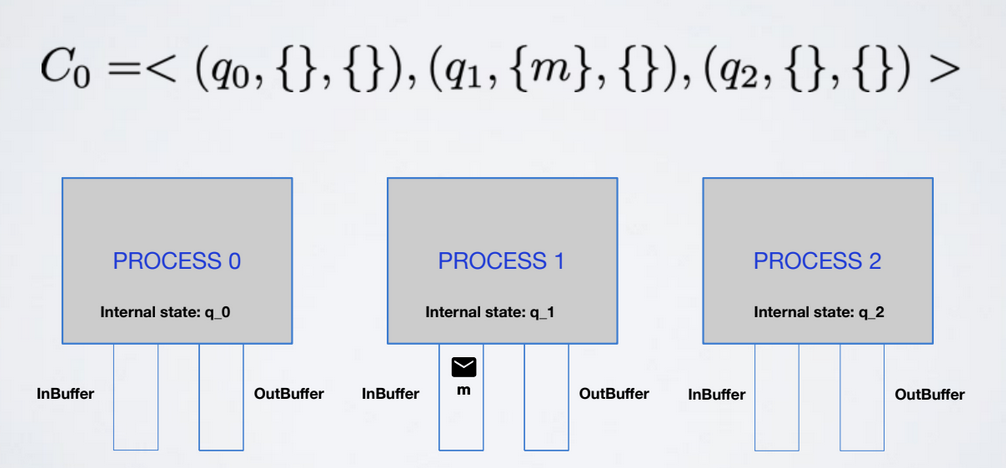
\includegraphics[scale=0.55]{img/configuration.png}
\end{center}
An event is \textbf{enabled} in configuration c if it can happen.
\begin{defn}
    An execution is an infinite sequence that alternates configurations and events: $(C_0,e_0,C_1,e_1,C_2,e_2,\dots)$ such that each event $e_t$ is enabled in configuration $C_t$ and $C_t$ is obtained by applying $e_{t-1} \text{ to } C_{t-1}$

\end{defn}
It may be useful to visualize how an execution involving multiple processes works, here we have an example:
\begin{center}
    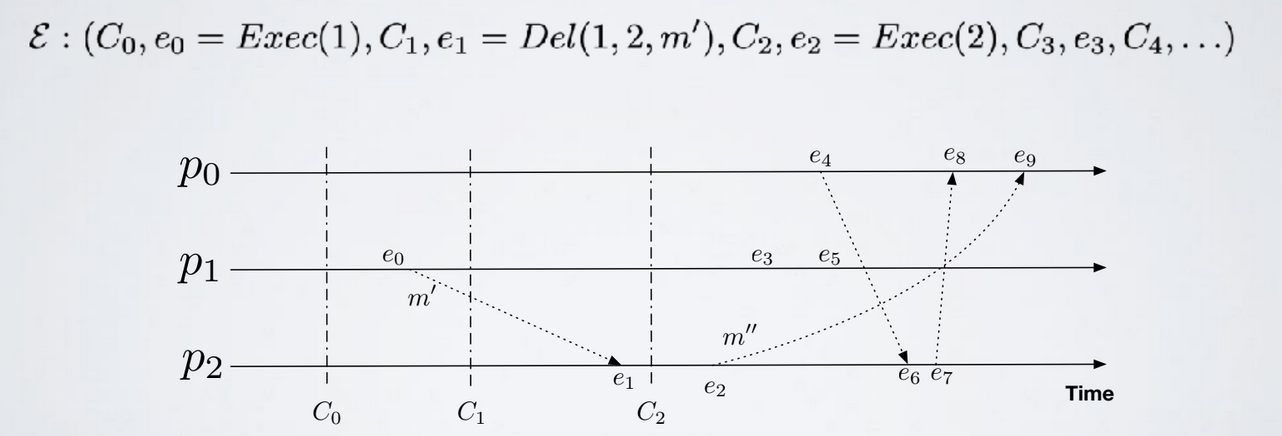
\includegraphics[scale=0.5]{img/execgraph.png}
\end{center}
\newpage
\begin{defn}
    A \textbf{fair execution} is an execution E where each process $p_i$ executes an infinite number of local computations (Exec(i) events are not finite) and each message m is eventually delivered (we can't stall messages)
\end{defn}
We will always use fair executions unless stated otherwise.
\begin{defn}
    Given an execution E and a procces $p_j$, we define the local view/ local execution of $E|p_j$ the subset of events in E that impact $p_j$
    \begin{center}
        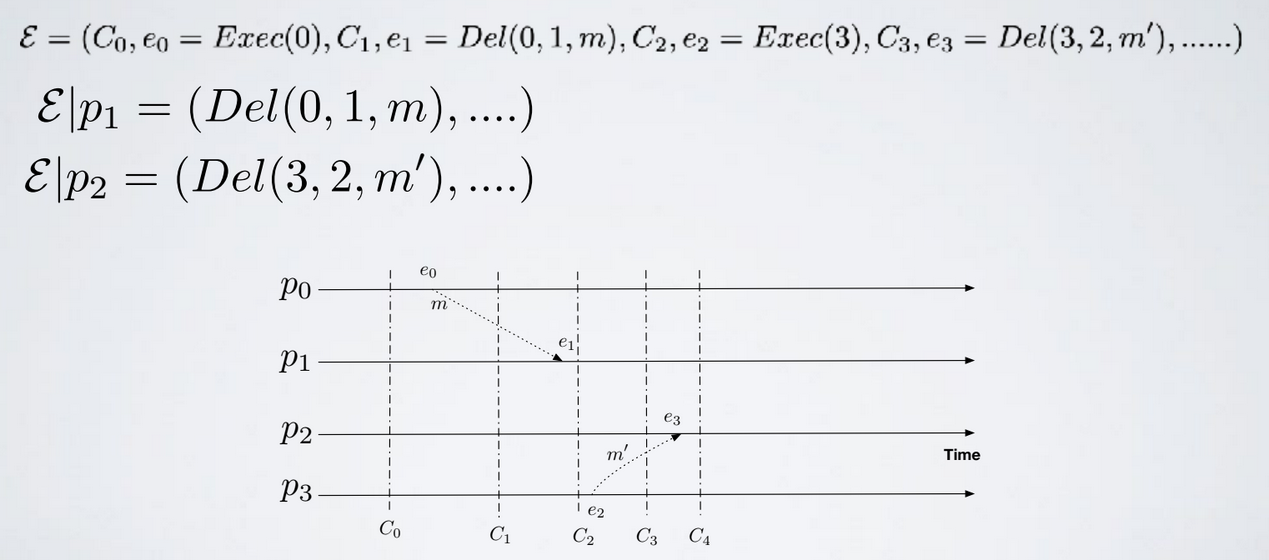
\includegraphics[scale=0.5]{img/localexec.png}
    \end{center}
\end{defn}
But these executions do not account for time, so we may have executions that are the same even though the events happened at different times, in case this does happen, we say that two executions are \textbf{\textit{indistinguishable}}.
\begin{thm}
In the asynch. model there is no distributed algorithm capable of reconstructing the system execution.
\end{thm}

\subsection{Synchronous Vs Asynchronous}
We have 3 main types of synchrony:
\begin{itemize}
    \item Asynchronous Systems
    \item Eventually Synchronous Systems
    \item Synchronous systems
\end{itemize}
We can say that is a system is synchronous if it has a fixed bound on the daly of messages, on the time of actions executed by processes, and a fixed bound between execution of actions.
\subsection{Failures}
We have 2 main models for failures:\\
\begin{itemize}
    \item Crash-stop Failures (The program crashes, and doesnt respond)
    \item Byzantine Failures (The behaviour of the program is random)
\end{itemize}
We signal crash failures with a star sign and byzantile failures with a !
\begin{center}
    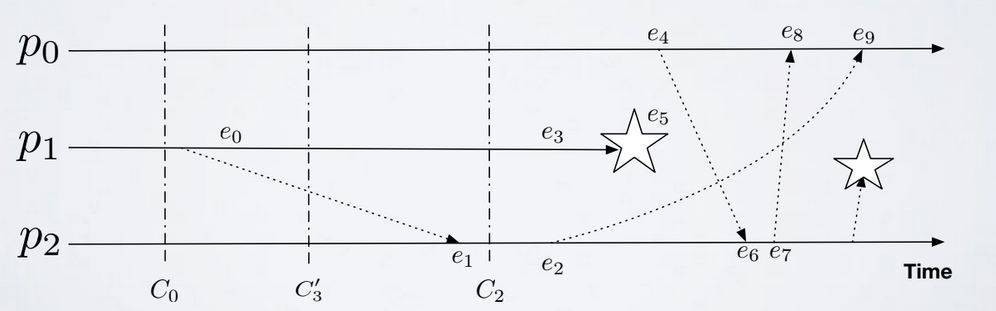
\includegraphics[scale=0.6]{img/crash.png}\\
    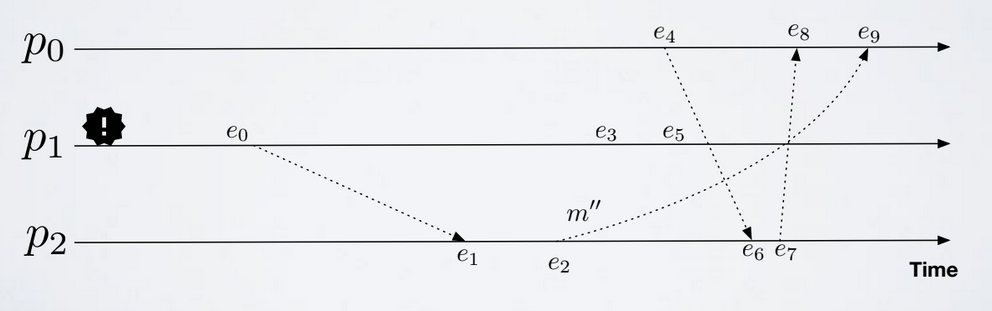
\includegraphics[scale=0.6]{img/byz.png}
\end{center}
Byzantine failures are a superset of Crashstop failures, so algorithms that will work on byzantine failures will always work on crash stop failures, but not the contrary.\\
A process is \textbf{correct} if it does not experience a failure, every algorithm has a maximum number f of failures that i can experience.

\subsection{Different types of links}

\begin{defn}
    An \textbf{Abstraction} is the formalization of a problem/object, to built one we must define the system model and formalize a problem/object so that there is no ambiguity regarding the properties of our abstraction
\end{defn}
For example let us abstract a link: it is something that may lose a message with a certain probability $pr$, the messages can be duplicated a finite number of times and they must come from somewhere.\\
Inside a link we have two main eents:
\begin{itemize}
    \item \textbf{Requests}: $<$Send | q,m$>$ sends message m to process q
    \item \textbf{Indication}: $<$Deliver | p,m$>$ delivers a message m from process p (this might just be an indetifier, e.g. an ip adress or mac address)
\end{itemize}
Now let us formalize this further via its properties:
\begin{itemize}
    \item \textbf{FL1}: (Fair loss) If a correct process p sends infinetely often m, a process q then delivers m an infinite number of times. (e.g. suppose we have $\frac{1}{2}$ probability and we send it over 10 times, then the probability will be $1 - \frac{1}{2^{10}}$ as events are independentm aka if we try hard enough we get the message)
    \item \textbf{FL2}: (Finite duplication) if a correct process p send m a finite number of times to q, then q cannot deliver m an infinite number of times (wel'll receive a finite number of duplicated packets)
    \item \textbf{FL3}: (No creation) If a certain process q sends a message m with send(p),then m was sent by p to q
\end{itemize}
Our objective is hiding the probability behind infinity.\\
A link that respects these properties is called a Fair-lossy link, and its always behind 2 process p and q. We can broadly categorize these properties into two classes:
\begin{itemize}
    \item \textbf{Safety}: if a property is violated at time t, then it cannot be satisfied after that time t. So if in an execution E we violated a safety property, then there is a prefix E' of E such that any extension E' also violates the property, an example of safety property is: if we die, we canno resurrect.
    \item \textbf{Liveness}: these kind of properties cannot be violated in a finite execution, more formally, given an execution E that does not satisfy a liveness property, there is an extension of E that satisfies it, informally it just says that something good will eventually happen.
\end{itemize}
If for example we created a bound on FL2, then we have a safety property, as it cannot be extended, as a rule of thumb, if the property is infinite, then it is a liveness property.\\
Of course there exist badly written properties that try and write both types into a rule, however we should always decompose them (e.g q will eventually deliver and the delivery is unique, if we decompose it we have "q eventually delivers, m is delivered at most once")\\
We also have what we call \textbf{stubborn links}, which inherit FL3 and add:
\begin{itemize}
    \item \textbf{SL1}: (Stubborn delivery) if a correct process p sends m to q, then q delivers m an infinite number of times, hence stubborn.

\end{itemize}
\begin{center}
    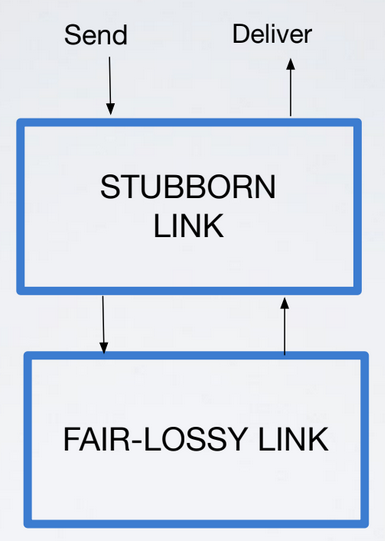
\includegraphics[scale=0.5]{img/links/sl.png}
\end{center}
Our algorithms will always reflect a reactive computing model utilizing handles that consume events or create them, they will always be atomic unless stated otherwise.
\begin{center}
    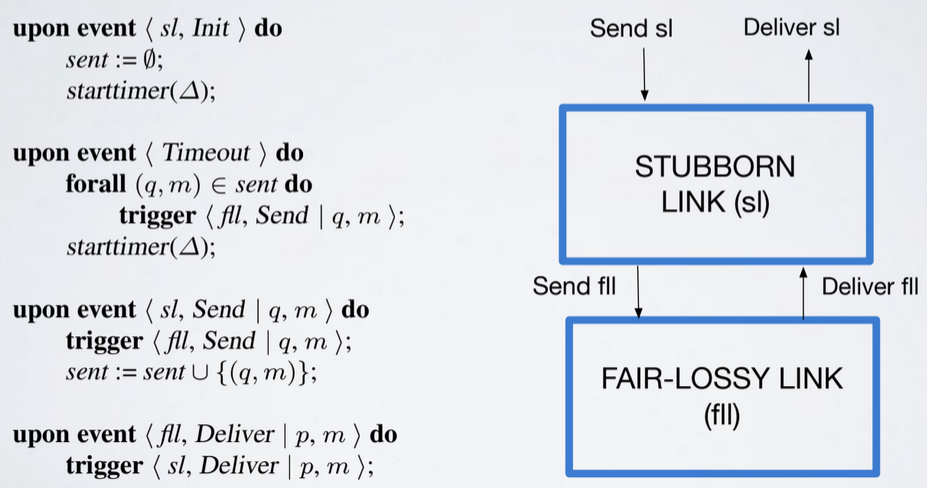
\includegraphics[scale=0.6]{img/links/slalgo.png}
\end{center}
The initialization event creates a set \textit{sent} containing the messages that were sent and then it start a local timer of delta time (delta is whatever we want), we must remember that this timer is not a global clock, but local for that process.\\
In an sl link whenever we get an input we trigger an event to send the message to our fll link, after that we just add it to our set sent.\\
When the fll wants to send a message to a process it will trigger an sl deliver event.\\
When a timeout event happens we scan all the messages in the sent set and we send them again, after that we start a timer.
\\\\
Then we have our \textbf{Perfect P2P} links which inherit FL3 but add the following properties:
\begin{itemize}
    \item \textbf{PL1}: Reliable delivery, if a correct process p sends m to q, then q eventually delivers m
    \item \textbf{PL2}: No duplication, a message is delivered at most once.
\end{itemize}
\begin{center}
    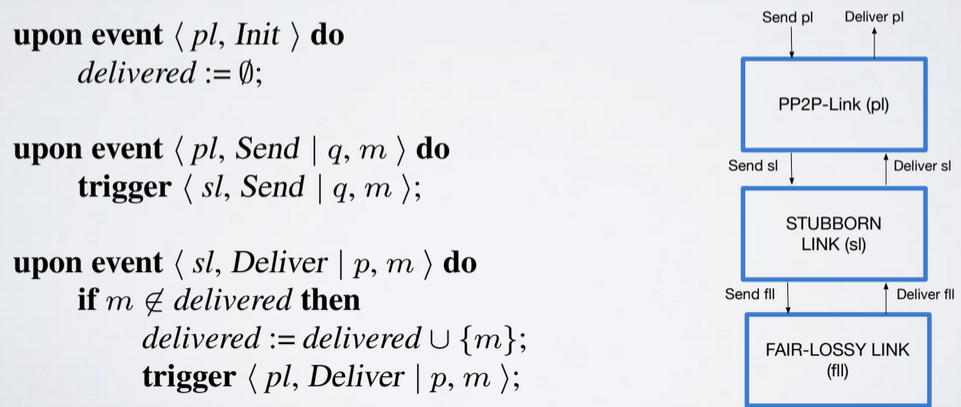
\includegraphics[scale=0.5]{img/links/p2p.png}
\end{center}
We initialize it with a delivered empty set, when we want to send a message we create an event and trigger a send event on the sl.\\
When the sl gets a deliver event we check if m is not delivered, else add it to delivered set, afer that we trigger a pl deliver event.\\\\
\textbf{Proof of no Duplication P2P}\\
Suppose we send m once, and you receive it twice, the delivery action of a message is guarded by “if m $\in$ delivered”, still suppose we deliver it twice at t' and t (t $<$ t'), however since the handler is atomic, we have that the set of delivered obtains message m, and therefore when m at t' is checked at time t' it is already in delivered, therefore it cannot be delivered again, as this contradicts the fact that trigger $<$pl,deliver $|$ P,m$>$ is executed at (or after) time t'.
\\\\
\textbf{PL1 Proof}\\
Suppse p sends m and q does not deliver it. There could be two reasons for q to not deliver:\\
Reason 1: You receive the message from the stubborn link and you drop it.\\
Reason 2: You don't receive a message m.\\
If q delivers a message then we execute the handler, the only way to not trigger $<$pl,Deliver$>$ is if it's the if m is $\in$ delivered, but someone must have delivered it already.\\
For the second reason we don't get a message at all, but the stubborn link has in turn properties that it cant violate, therefore it is impossible, since the delivery handler would never be triggered.\\\\
\textbf{Exercise 1}\\
Show that our stubborn algorithm does not work if we change first property to:\\
\textit{SL(1) If a process p sends m to q, then q delivers m an infinite number of times}\\
Whats missing is the word “correct” therefore the process may crash, so our algorithm with a timer does not work.\\
Suppose we want to implement this then:\\
If a process p sends a message m to q, then q delivers m 1 time. Suppose we also have a perfect channel that we need to deliver message m to, but since the process is still not correct, then our link may receive the message and crash, or even before it receives it, it crashes. Therefore it cant be done.
\section{Time in Distributed Systems}
We have different type of "times" in DS:
\begin{itemize}
    \item \textbf{Asynchronous}: No Global-clock, no bound,local-computational steps (Exec) happen at unpredictable time (the adversary e.g. the scheduler), models everything but has a lot of problems
    \item \textbf{Synchronous}: Bound, you can synchronize up to a certain precision, local execution steps happen at certain predetermined interval, and they take a bounded time, models only networks but everything is possible
    \item \textbf{Eventually Synchronous}: we have a threshold, where if its under its under its in sync, else its async. In an eventually synchronous a safety property does not work  if it depends on the delay of the channel.
\end{itemize}
\subsection{Clock Synchronization}
To actually work most applications need an order of actions and synchronization.\\
To synchronize we need a clock, this clock on most computers works by  measuring the oscillation and a counting register that is incremented at every tick of the oscillator, at certain times the OS reads the hardware clock $H_i (t)$ and produces the local software clock $C_i (t) = \alpha * H_i (t) + \beta$.
The hardware clock is: $$ H_i (t) = \int_{0}^{t} h_i(\tau)d\tau$$
Between two clocks we may have a \textbf{skew} , which is the $|C_i (t) - C_j (t)|$, we may also have a \textbf{drift rate} which is the gradual misalignment of synchronized clocks caused by slight inaccuracies of time-keeping mechanisms, more formally it is the derivate of the hardware clock over the derivative of the time.
\begin{center}
    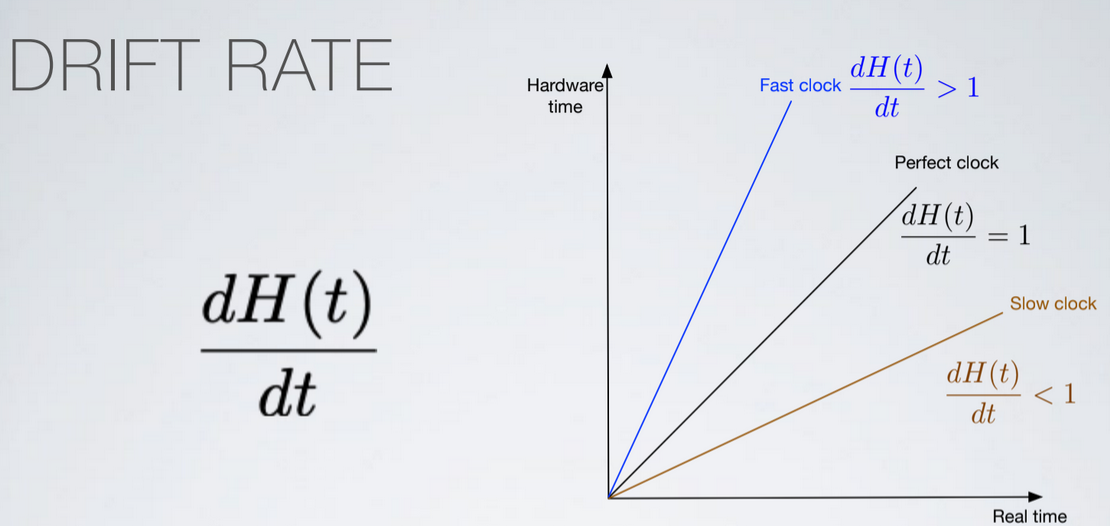
\includegraphics[scale=0.5]{img/clocks/dr.png}
\end{center}
To synchronize two clocks we have 2 strategies, either bring one in the future or bring it in the past by modifying beta, we never go into the past as we may have done something before the sync and it would cause confusion. We can however slow the clock that is in the future.
\begin{center}
    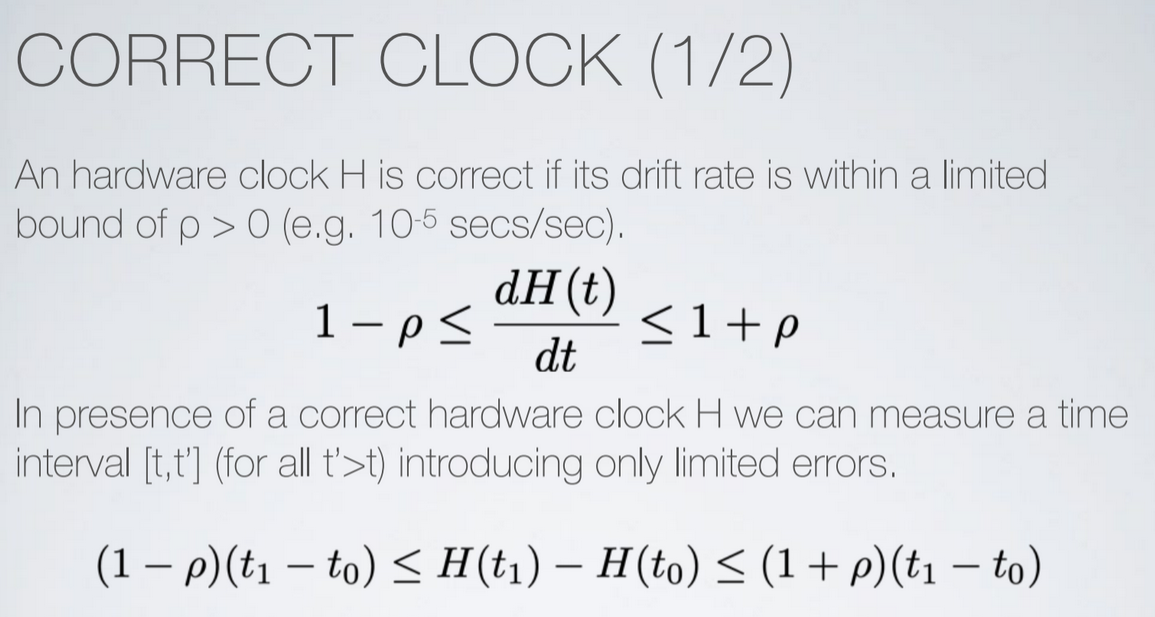
\includegraphics[scale=0.5]{img/clocks/cc1.png}
    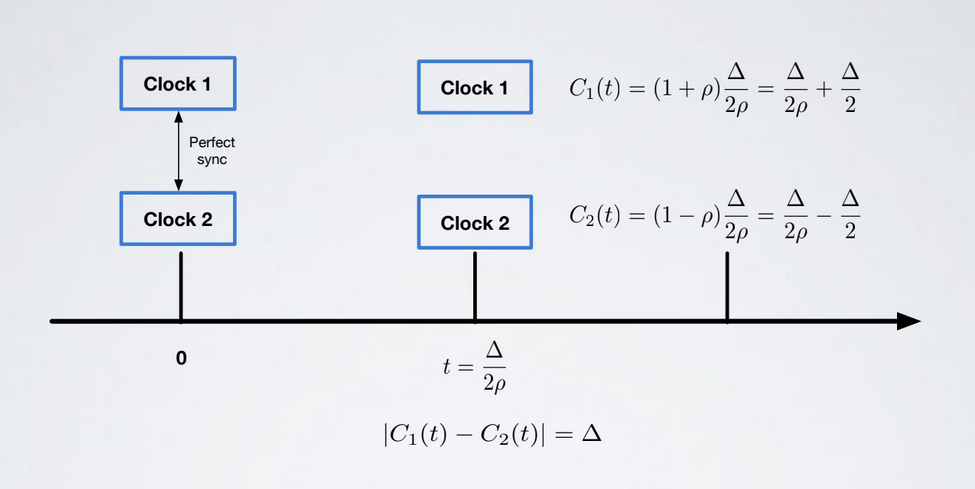
\includegraphics[scale=0.6]{img/clocks/cc2.png}
    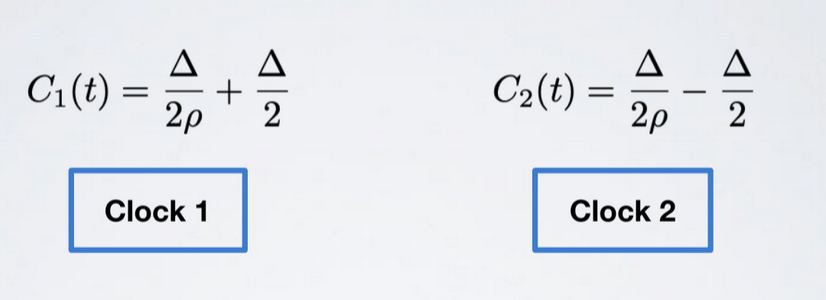
\includegraphics[scale=0.7]{img/clocks/cc3.png}
    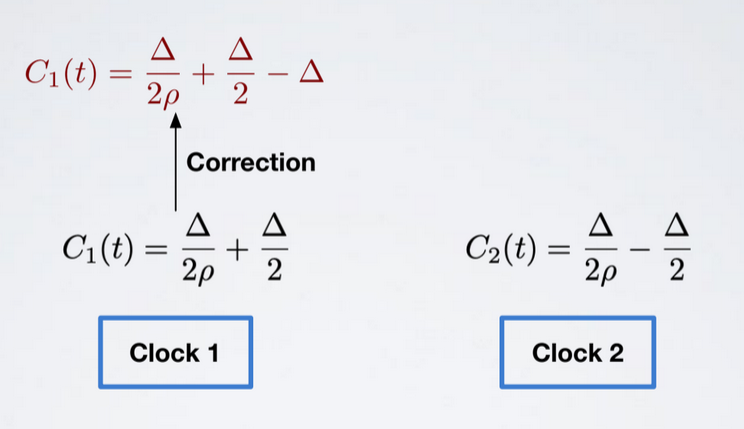
\includegraphics[scale=0.7]{img/clocks/cc4.png}
\end{center}
All software clocks have to be monotone:
$$ t' > t \implies C(t') > C(t)$$
So if real time t' is greater than t, we have that the software clocks reflect that, to actually reflect this, we cannot choose a value $\beta$ in the negatives, but rather
a value $\alpha$ that is $<$ 1 by \textit{masking oscillations} as well changing the value $\beta$.\\
When we synchronize with external time, we synchronize with UTC as it is the international standard and we'll synchronize via satellites.\\
We can define \textbf{external synchronization} when we synchro with UTC, so each process is synchronized with an authorative external source, this means that the difference between any computer and the external source is below a certain bound D.\\
If we don't synchro with the external world we are doing \textbf{Internal synchronization}, a set of processes is internally synchronized if the difference between their clocks is less than D. If we have external we also have internal.
\subsection{Algorithms for synchronization}
For external synchronization we have christian's algorithm, we utilize a Server S that receives a signal from an UTC source, works (probabilistically) in async systems, its based on RTTs, and only if RTTs are small and respect the required accuracy will the response be considered. We can also divide  to know the difference between when the server sent the info and when I received it, so just add $time\_ response + \frac{RTT}{2}$ but this assumes that RTT is symmetric.
Another problem is the fact that we have a single point of failure (server) in real life we just synchronize with multiple servers.
\begin{center}
    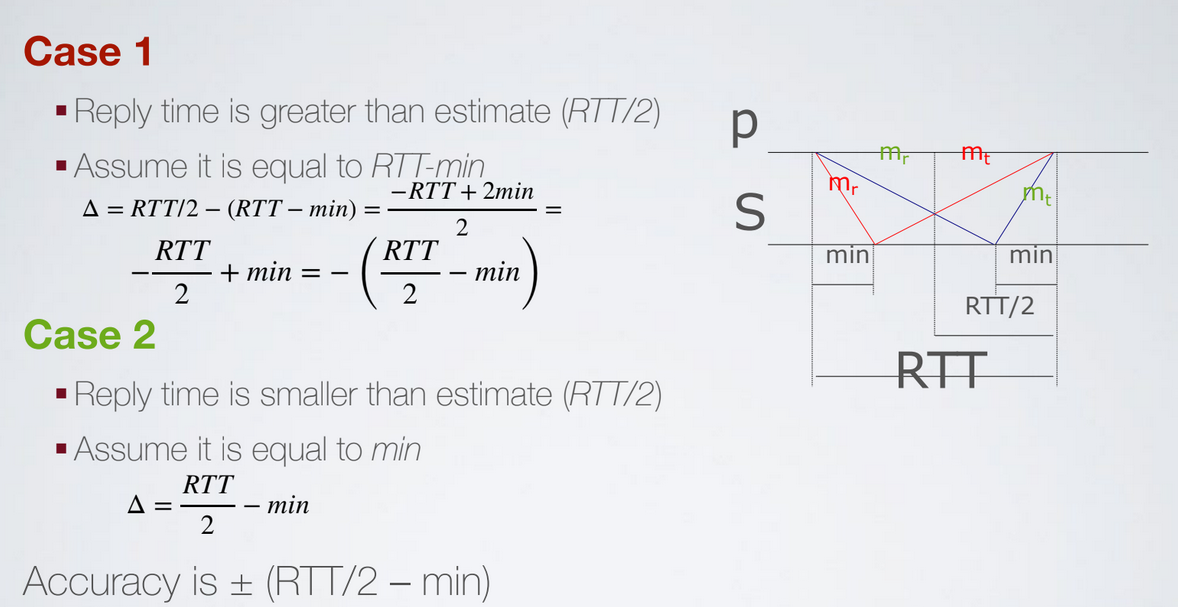
\includegraphics[scale=0.5]{img/synchro_algs/image.png}
\end{center}

\end{document}